\Annex{Annexe sur l'évaluation d'un \textit{clustering} à l'aide de la \texttt{v-measure}}
\label{annex:D-ANNEXE-EVALUATION-CLUSTERING}

	% INTRODUCTION DE L'ANNEXE.
	\todo[inline]{à rédiger}

	% TABLE DES MATIÈRES DE L'ANNEXE.
	\minitoc

	%%%%%--------------------------------------------------------------------
	%%%%% Annexe D.1: Définition de la \texttt{v-measure}.
	%%%%%--------------------------------------------------------------------
	\section{Définition de la \texttt{v-measure}}
	\label{annex:D.1-ANNEXE-EVALUATION-CLUSTERING-DEFINITION}
	\todo[inline]{ANNEXE: v-measure}
	
		%%% Description générale.
		
		%%% Formulation mathématique.
		
		% Notations.
		Pour la suite de l'exposé, nous allons utiliser les notations suivantes :
		\begin{itemize}
			% Data.
			\item $\mathcal{D}$ représente l'ensemble des données $d$ à segmenter ;
			% Classes.
			\item $\mathcal{C}$ représente l'ensemble des classes $c$ possibles de la segmentation de référence, et $\texttt{classe}[d]$ représente la classe d'une donnée $d \in \mathcal{D}$ ;
			% Clusters.
			\item $\mathcal{K}$ représente l'ensemble des \textit{clusters} $k$ possibles de la segmentation, et $\texttt{cluster}[d]$ représente le \textit{cluster} d'une donnée $d \in \mathcal{D}$ ;
		\end{itemize}
		
		% Equation.
		\begin{equation}
			\label{equation:D.1-ANNEXE-EVALUATION-CLUSTERING-DEFINITION-ENTROPTY-DUO}
			H(C|K)~=~
				-
				\sum\limits_{
					c \in \mathcal{C}
				}
				\sum\limits_{
					k \in \mathcal{K}
				}
				\frac{
					|c \cap k|
				}{
					|\mathcal{D}|
				}
				\cdot
				\texttt{log} \biggl(
					\frac{
						|c \cap k|
					}{
						|k|
					}
				\biggr)
		\end{equation}
		
		% Equation.
		\begin{equation}
			\label{equation:D.1-ANNEXE-EVALUATION-CLUSTERING-DEFINITION-ENTROPTY-SOLO}
			\begin{cases}
				H(C)
					& =
					-
					\sum\limits_{
						c \in \mathcal{C}
					}
					\frac{
						|c|
					}{
						|\mathcal{D}|
					}
					\cdot
					\texttt{log} \biggl(
						\frac{
							|c|
						}{
							|\mathcal{D}|
						}
					\biggr) \\
				H(K)
					& =
					-
					\sum\limits_{
						k \in \mathcal{K}
					}
					\frac{
						|k|
					}{
						|\mathcal{D}|
					}
					\cdot
					\texttt{log} \biggl(
						\frac{
							|k|
						}{
							|\mathcal{D}|
						}
					\biggr)
			\end{cases}
		\end{equation}
		
		% Equation.
		\begin{equation}
			\label{equation:D.1-ANNEXE-EVALUATION-CLUSTERING-DEFINITION-HOMEGENEITE-COMPLETENESS}
			\begin{cases}
				\texttt{homogeneity}(C|K)
					& =
					1
					-
					\frac{
						H(C|K)
					}{
						H(C)
					} \\
				\texttt{completeness}(C|K)
					& =
					1
					-
					\frac{
						H(K|C)
					}{
						H(K)
					} \\
				\texttt{homogeneity}(C|K)
					& = \texttt{completeness}(K|C)
			\end{cases}
		\end{equation}
		
		% Equation.
		\begin{equation}
			\label{equation:D.1-ANNEXE-EVALUATION-CLUSTERING-DEFINITION-VMEASURE}
			\texttt{v-measure}(C|K)~=~2 \cdot \frac{
				\texttt{homogeneity}(C|K) \cdot \texttt{completeness}(C|K)
			}{
				\texttt{homogeneity}(C|K) + \texttt{completeness}(C|K)
			}
		\end{equation}

	%%%%%--------------------------------------------------------------------
	%%%%% Annexe D.2: Quelques exemples de calcul avec la \texttt{v-measure}.
	%%%%%--------------------------------------------------------------------
	\section{Quelques exemples de calcul avec la \texttt{v-measure}}
	\label{annex:D.2-ANNEXE-EVALUATION-CLUSTERING-EXEMPLE-VMEASURE}
	\todo[inline]{ANNEXE: v-measure}
	
		% Exemple 0:
		\begin{figure}[H]
			\centering
			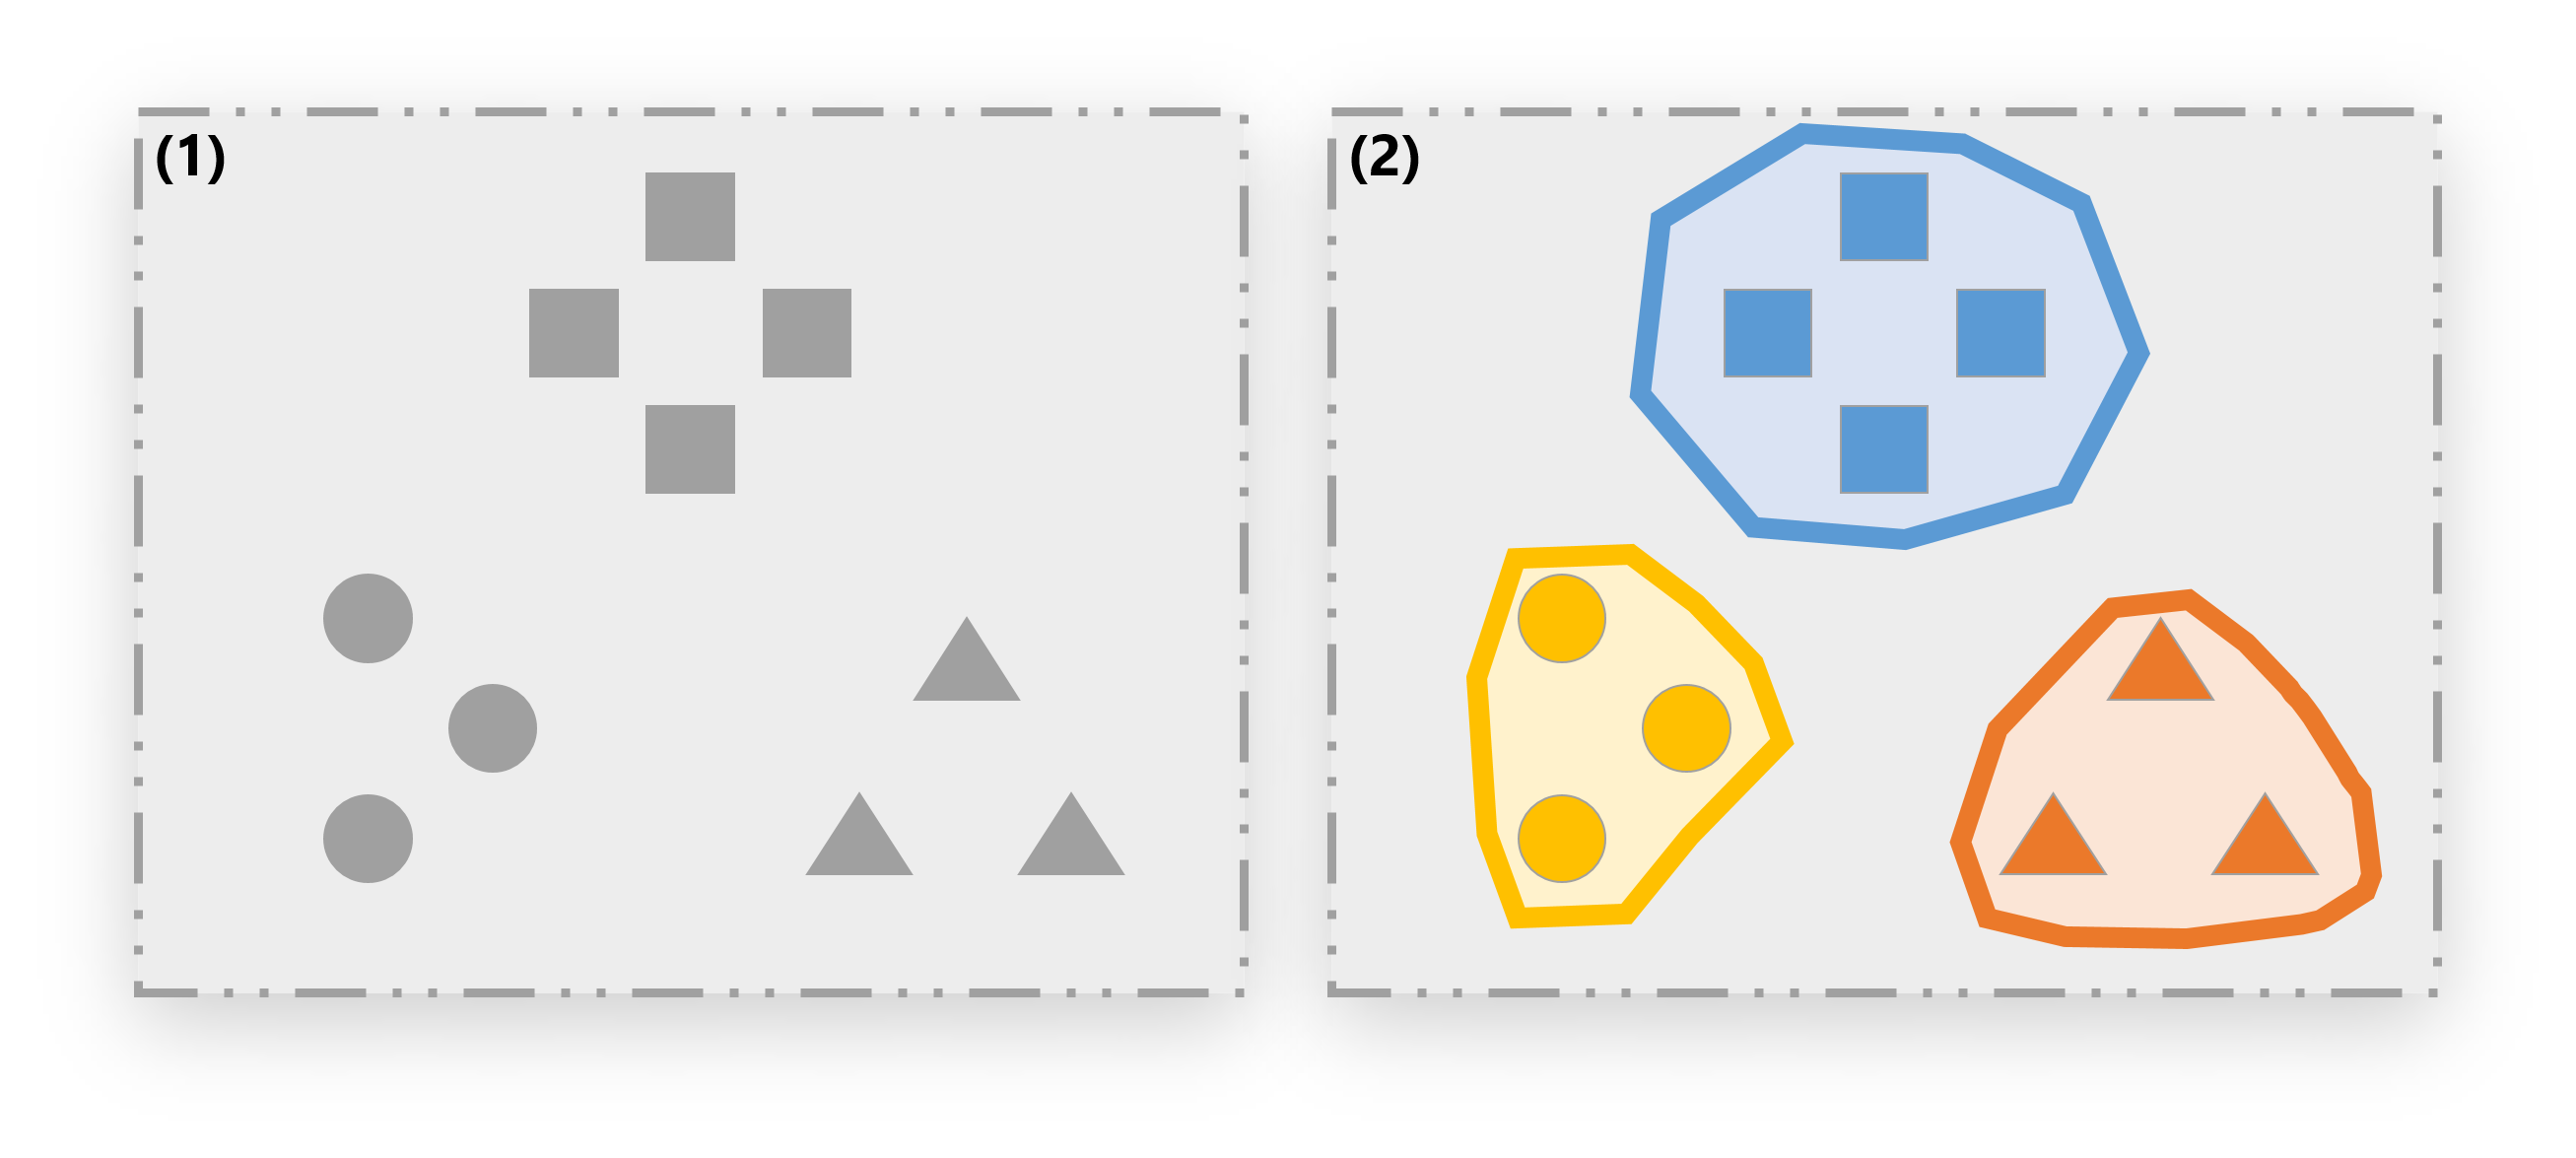
\includegraphics[width=0.95\textwidth]{figures/annexe-vmeasure-presentation}
			\caption{
				Présentation du jeu d'exemple :
				\textbf{(1)} représente $10$ données non regroupées ;
				\textbf{(2)} représente ces $10$ données regroupées en $3$ \textit{clusters} en fonction de formes.
			}
			\label{figure:D.2-ANNEXE-EVALUATION-CLUSTERING-EXEMPLE-VMEASURE-0-PRESENTATION}
		\end{figure}
			%
			\textsc{Figure~\ref{figure:D.2-ANNEXE-EVALUATION-CLUSTERING-EXEMPLE-VMEASURE-0-PRESENTATION}} \textbf{(1)}
			%
			\textsc{Figure~\ref{figure:D.2-ANNEXE-EVALUATION-CLUSTERING-EXEMPLE-VMEASURE-0-PRESENTATION}} \textbf{(2)}: $h = 1.00$, $c = 1.00$, $v = 1.00$.
	
		% Exemple 1:
		\begin{figure}[H]
			\centering
			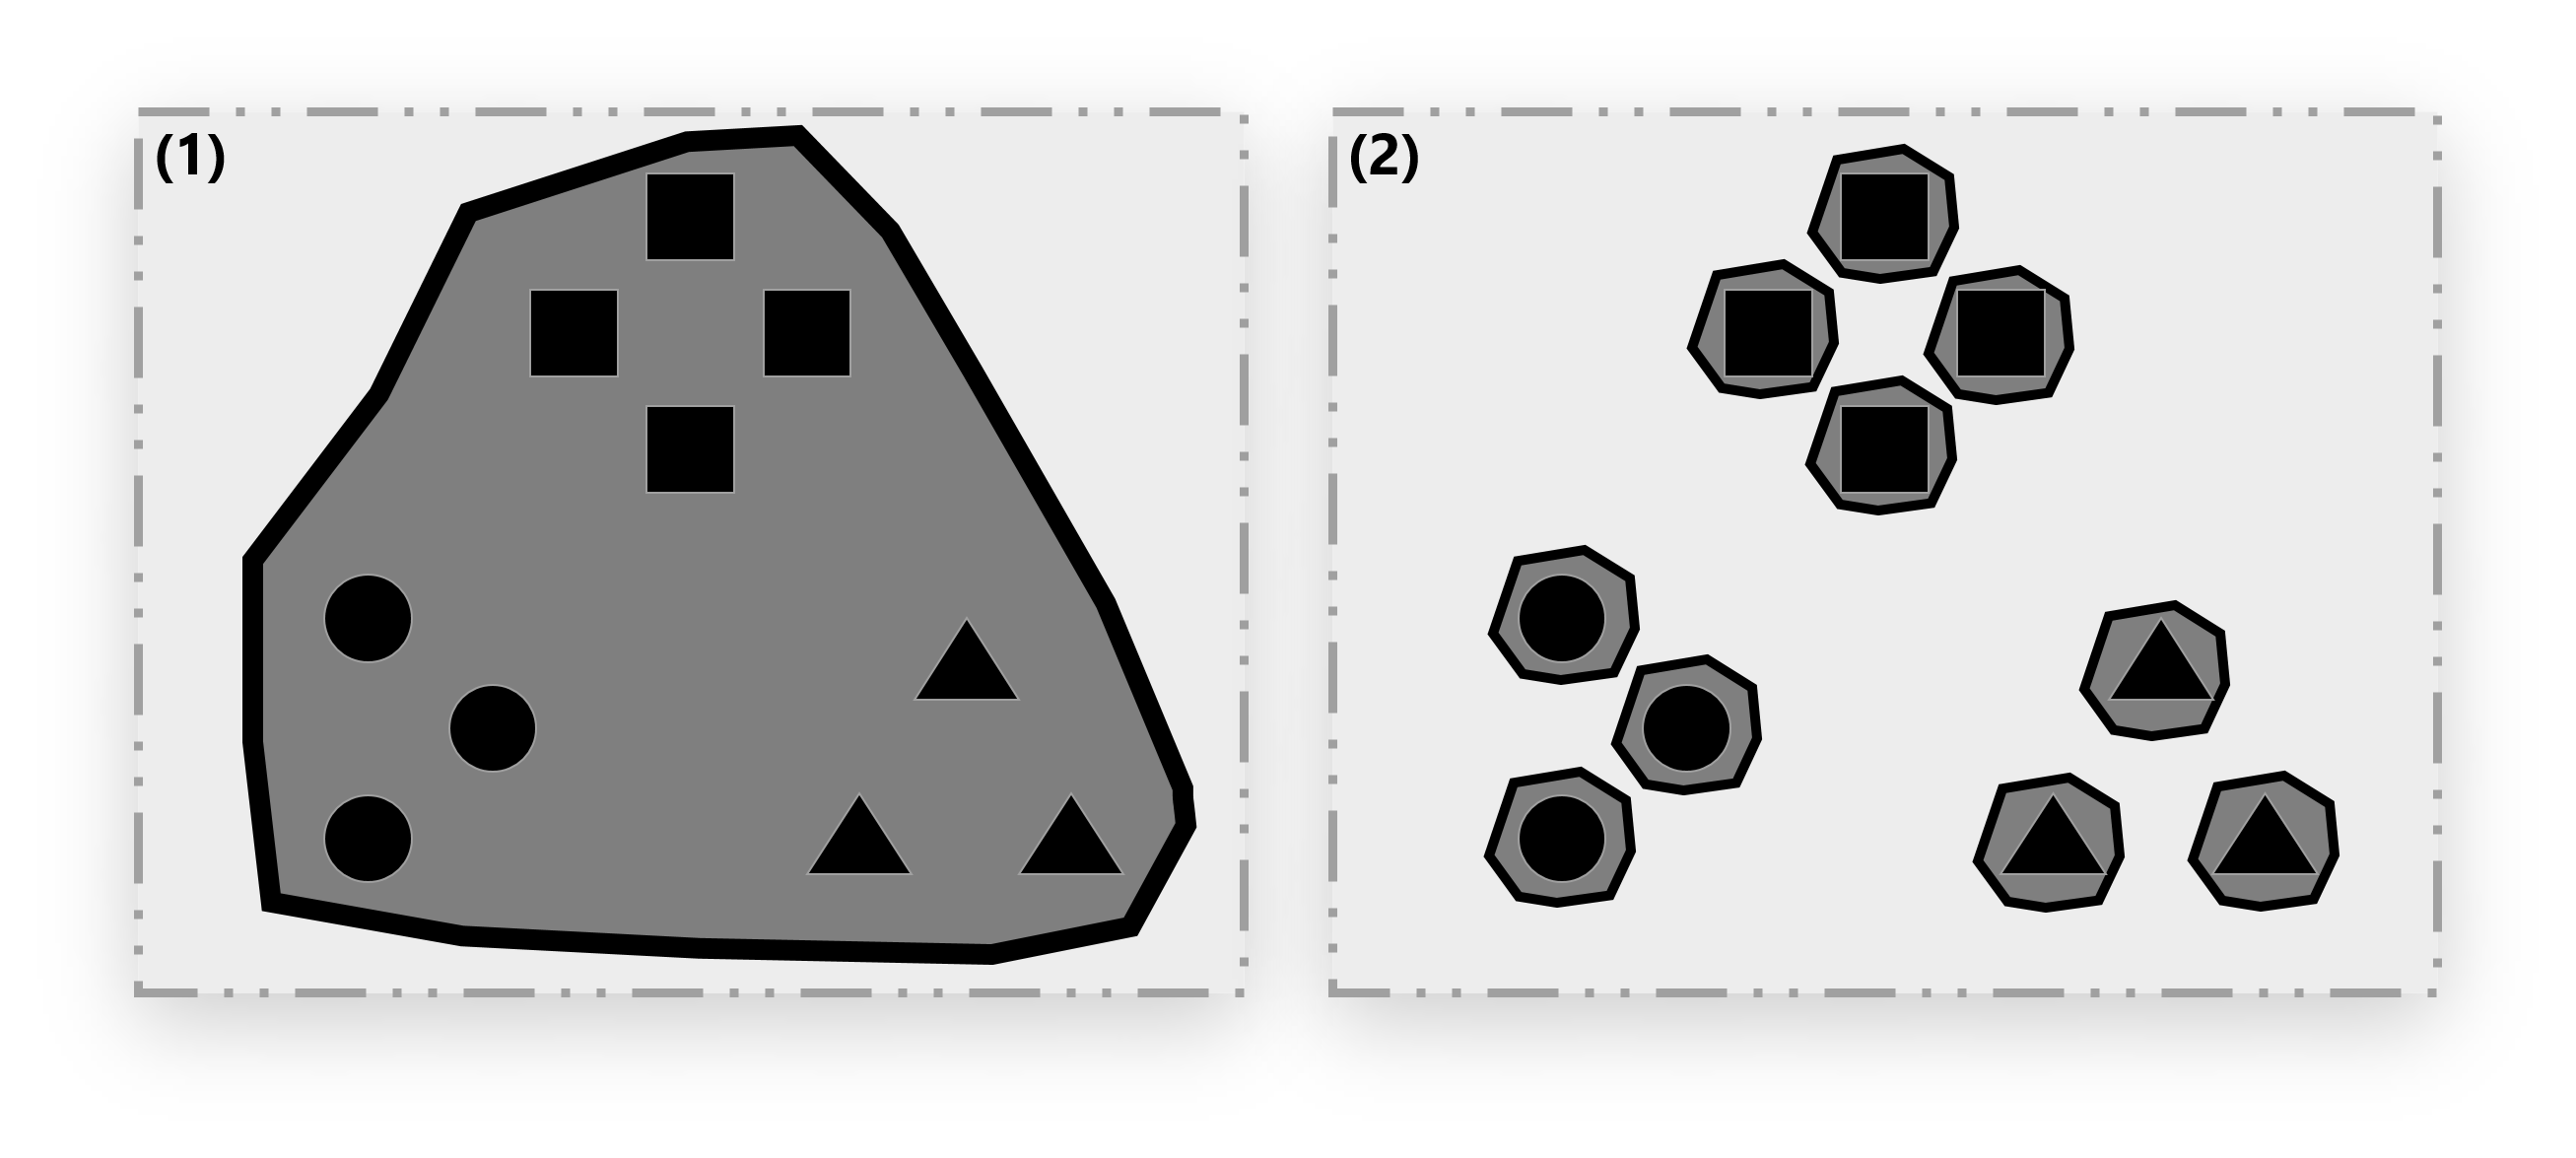
\includegraphics[width=0.95\textwidth]{figures/annexe-vmeasure-cas-extremes}
			\caption{
				Exemples de \texttt{clustering} avec des cas extrêmes :
				\textbf{(1)} représente un regroupement en $1$ \textit{cluster} où toutes les données sont contenues dans cet unique \textit{cluster} ;
				\textbf{(2)} représente un regroupement en $10$ \textit{clusters} où chaque \textit{cluster} contient une seule donnée.
			}
			\label{figure:D.2-ANNEXE-EVALUATION-CLUSTERING-EXEMPLE-VMEASURE-1-CAS-EXTREME}
		\end{figure}
			%
			\textsc{Figure~\ref{figure:D.2-ANNEXE-EVALUATION-CLUSTERING-EXEMPLE-VMEASURE-1-CAS-EXTREME}} \textbf{(1)}: $h = 0.00$, $c = 1.00$, $v = 0.00$.
			%
			\textsc{Figure~\ref{figure:D.2-ANNEXE-EVALUATION-CLUSTERING-EXEMPLE-VMEASURE-1-CAS-EXTREME}} \textbf{(2)}: $h = 1.00$, $c = 0.00$, $v = 1.00$.
	
		% Exemple 2:
		\begin{figure}[H]
			\centering
			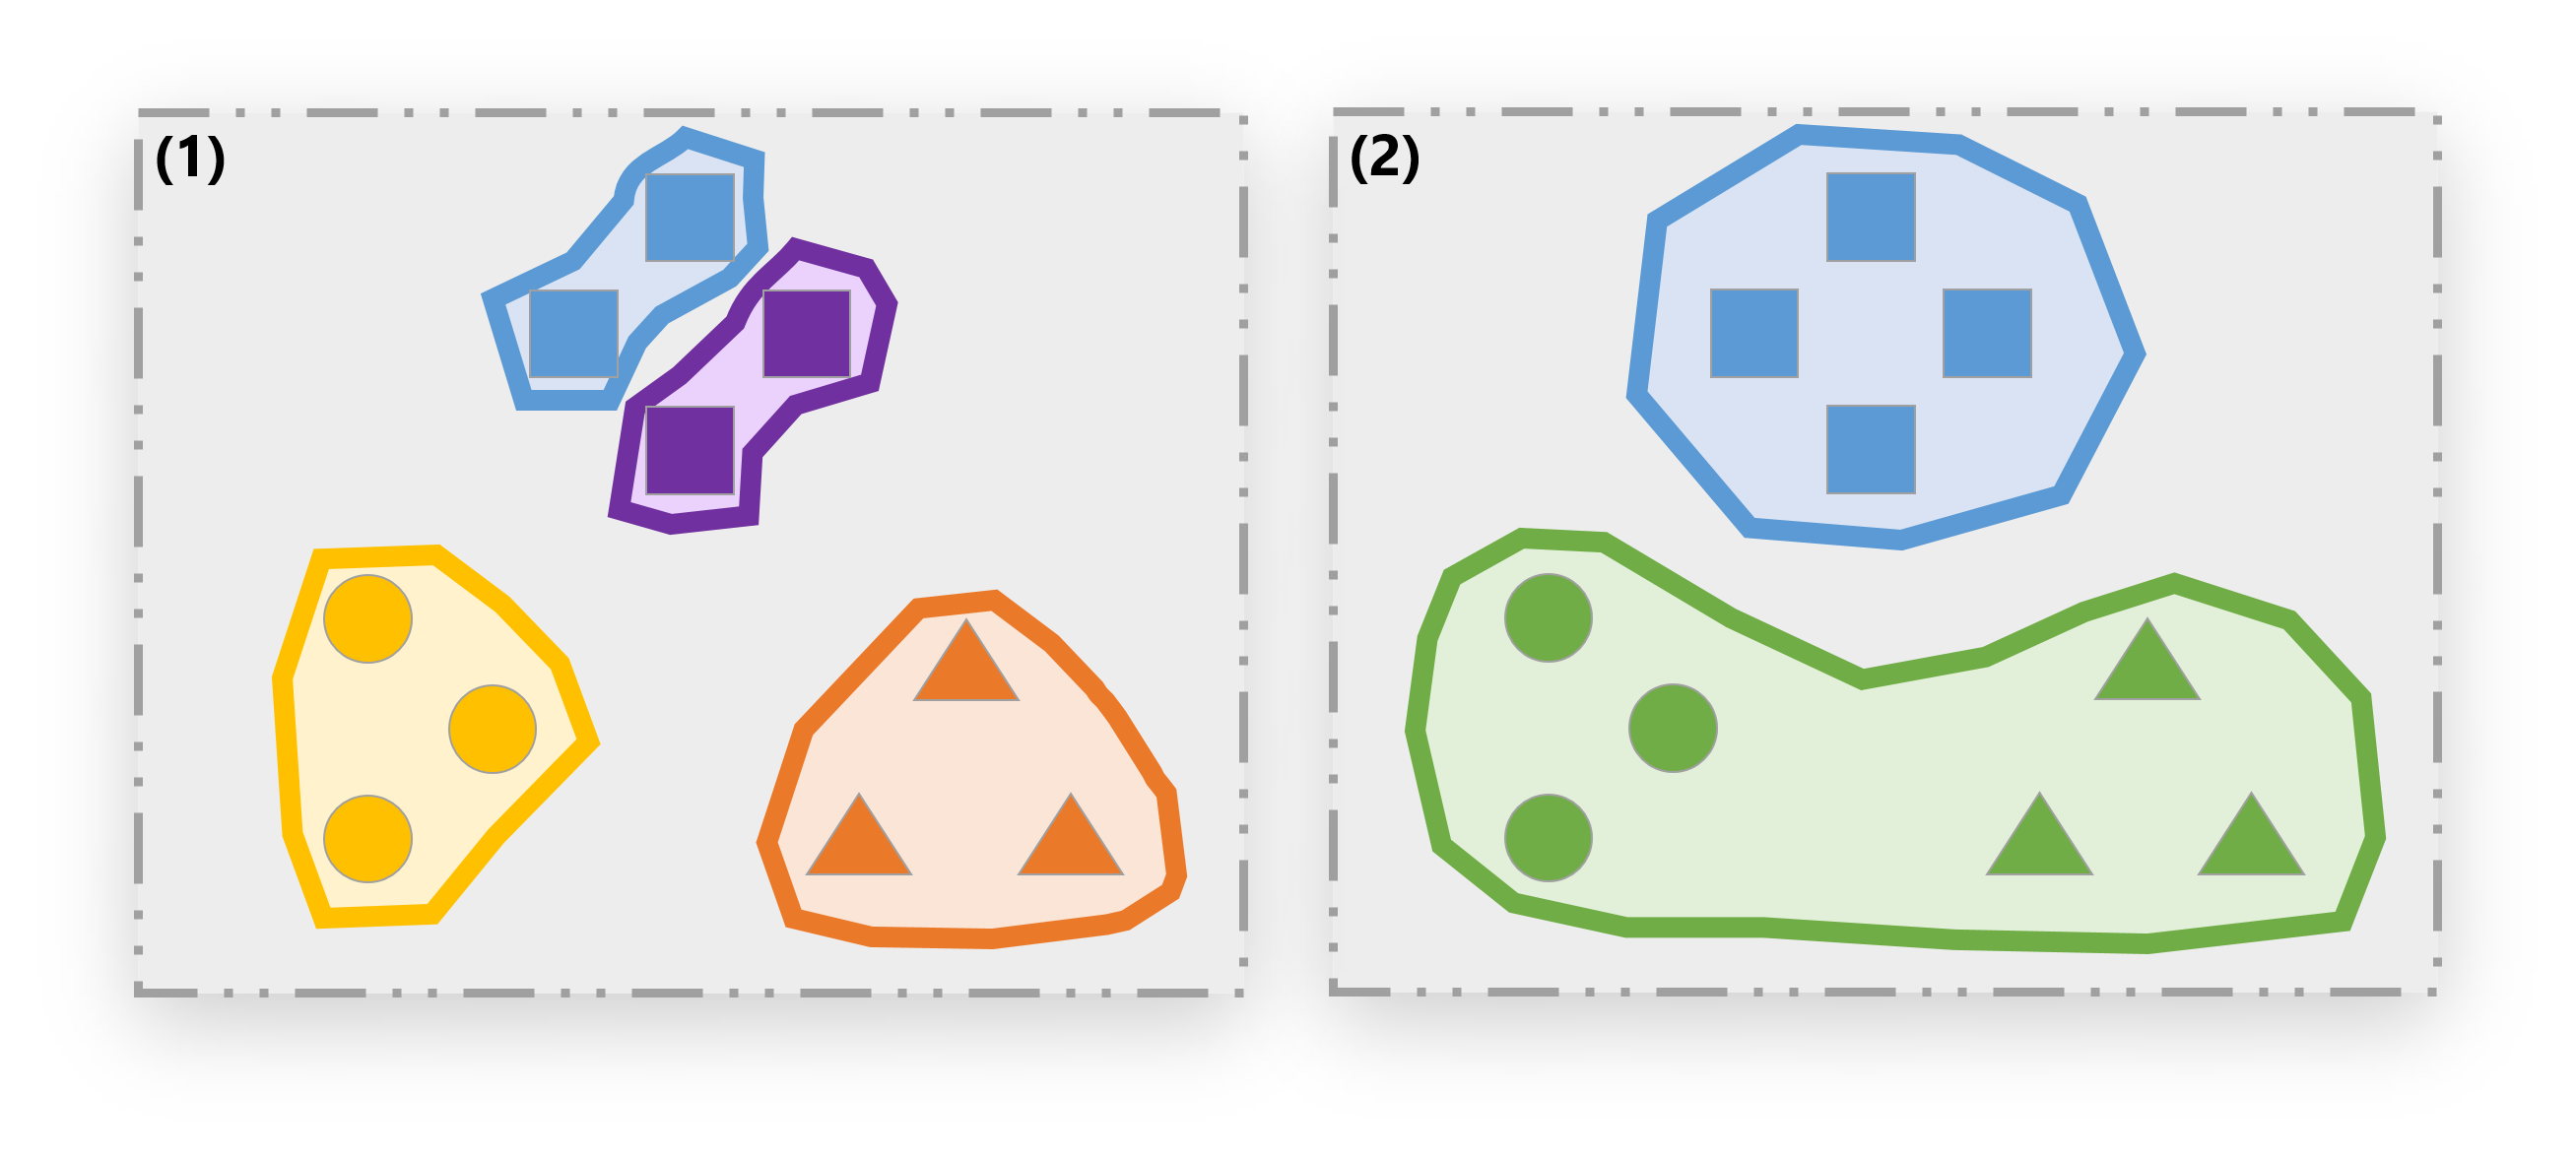
\includegraphics[width=0.95\textwidth]{figures/annexe-vmeasure-cas-simples}
			\caption{
				Exemples de \texttt{clustering} avec des cas simples :
				\textbf{(1)} représente un regroupement en $4$ \textit{clusters} où les rond et les triangles sont correctement regroupés, mais où les carrés sont séparés.
				\textbf{(2)} représente un regroupement en $2$ \textit{clusters} où les carrés sont correctement regroupés, mais où les ronds et les triangles ont été rassemblés.
			}
			\label{figure:D.2-ANNEXE-EVALUATION-CLUSTERING-EXEMPLE-VMEASURE-2-CAS-SIMPLES}
		\end{figure}
			%
			\textsc{Figure~\ref{figure:D.2-ANNEXE-EVALUATION-CLUSTERING-EXEMPLE-VMEASURE-2-CAS-SIMPLES}} \textbf{(1)}: $h = 1.00$, $c \propto 0.78$, $v \propto 0.89$.
			%
			\textsc{Figure~\ref{figure:D.2-ANNEXE-EVALUATION-CLUSTERING-EXEMPLE-VMEASURE-2-CAS-SIMPLES}} \textbf{(2)}: $h \propto 0.62$, $c = 1.00$, $v \propto 0.76$.
	
	